\chapter{Results}
\label{chap:results}

\setlength{\epigraphwidth}{1.0\textwidth}
\epigraph{The closer a machine translation is to a professional human translation, the better it is.}{--- Papineni et al., BLEU: a Method for Automatic Evaluation of Machine Translation}

% TODO: A short intro?

\section{Cs-En dataset}
\label{sec:cs-en-results}

We performed 14 experimental phrase table extractions for Cs-En dataset,
the comprehensive list is presented by \Tref{cs-en-wmt13-scenarios}.
We included one more optimized baseline with 8 cores, because the difference in
wall clock time necessary to construct the phrase table between runs with 4 and 8 cores
was considerable.
Sorting processes in both optimized baselines were given 18~GB of memory, so the virtual
peak of entire pipeline reached approximately the same value as in case of \eppex{}
run with no pruning.

% Cs-En: description and parameters of experiments
\begin{table}[ht]
\centering
\begin{tabular}{ r p{10cm} }
name & description and parameters \\
\hline
\hline
def-base        & Standard Moses pipeline with no special parameters \\
multi-base      & Standard Moses pipeline with \verb|--cores 4| \\
comp-base       & Standard Moses pipeline with \verb|--sort-compress gzip| and \verb|--cores 4| \\
opt-base        & Standard Moses pipeline with \verb|--sort-buffer 18G|, \verb|--sort-compress gzip| and \verb|--cores 4| \\
opt-c8-base     & Standard Moses pipeline with \verb|--sort-buffer 18G|, \verb|--sort-compress gzip| and \verb|--cores 8| \\
\hline
eppex zero      & \eppex{} set to no pruning and \verb|--GZOutput| option \\
eppex def.      & \eppex{} with \verb|--limits| set to \verb|1-3:0:1,4-5:1:4,6-7:4:8| and \verb|--GZOutput| option \\
eppex 0:n       & \eppex{} with \verb|--limits| set to \verb|1:0:1,2:0:2,...,7:0:7| and \verb|--GZOutput| option \\
eppex 0:n+1     & \eppex{} with \verb|--limits| set to \verb|1:0:2,2:0:3,...,7:0:8| and \verb|--GZOutput| option \\
eppex 1:n+1     & \eppex{} with \verb|--limits| set to \verb|1:1:2,2:1:3,...,7:1:8| and \verb|--GZOutput| option \\
\hline
sigfilter a-e   & baseline followed by significance filtering with pruning threshold $\alpha - \epsilon$ \\
sigfilter a+e   & baseline followed by significance filtering with pruning threshold $\alpha + \epsilon$ \\
sigfilter 30 a+e  & baseline followed by significance filtering with cutoff limit of 30 and pruning threshold $\alpha + \epsilon$ \\
sigfilter 30    & baseline followed by significance filtering with cutoff limit of 30 \\
\hline
\hline
\end{tabular}
\caption{\label{cs-en-wmt13-scenarios}
List of various experiments and their settings for Cs-En setup, "eppex~def." is shortcut for \emph{eppex defensive}.}
\end{table}

The \emph{eppex zero} experiment is performed to establish the maximum memory demands of \eppex{}
for the input data of a given size.
The \emph{eppex defensive} experiment has the positive and negative limits set to achieve the same
level of pruning as the \emph{eppex 1-in} experiment that performed very well in 2011 experiments.
The remaining \eppex{} experiments have a separate Lossy Counter set for every phrase length:
the negative limit is the same for all instances, but the positive limit is set in correspondence
to a phrase length to allow for a bigger estimation errors in the case of longer phrase pairs.

\subsection{Translation phrase table size and quality}

\Tref{cs-en-wmt13-pt-size-and-bleu} presents the phrase table sizes and BLEU scores for all
distinct phrase tables created in our experiments.
Despite that the phrase table sizes are very different, with the most pruned phrase table being
only $1/13$ size of the baseline, the achieved BLEU scores are very tight and the difference
between the best and the worst score is only 0.66~point in the case of \emph{news-test2012} test data
and 0.61~point in the case of \emph{news-test2013} test data.

% Cs-En: phrase tables sizes and BLEU scores
\begin{table}[ht]
\centering
\begin{tabular}{ | c | c c | c c | }
\hline
 & \multicolumn{2}{|c|}{final phrase table size} & \multicolumn{2}{|c|}{BLEU score} \\
experiment & phrase pairs & .gz file size & wmt-12 & wmt-13 \\
\hline
\hline
baseline          & 336.0~M & 8.8~GB & 23.27 & 25.83 \\
sigfilter 30      & 301.9~M & 8.2~GB & 23.12 & 25.62 \\
sigfilter a-e     & 203.1~M & 5.9~GB & 23.01 & 25.60 \\
eppex def.        & 109.8~M & 2.7~GB & \textbf{23.38} & \textbf{25.98} \\
eppex 0:n         &  86.2~M & 2.3~GB & 23.24 & 25.86 \\
sigfilter a+e     &  70.0~M & 1.9~GB & 23.21 & 25.59 \\
eppex 0:n+1       &  67.9~M & 1.8~GB & 23.04 & 25.61 \\
sigfilter 30 a+e  &  60.2~M & 1.7~GB & 23.05 & 25.63 \\
eppex 1:n+1       &  25.7~M & 0.7~GB & 22.72 & 25.37 \\
\hline
\end{tabular}
\caption{\label{cs-en-wmt13-pt-size-and-bleu}
Phrase table sizes and BLEU scores for the various experiments of Cs-En setup.}
\end{table}

The \emph{eppex defensive} experiment again proved to be very competitive:
the phrase table has only $1/3$ of size of the baseline,
but the obtained BLEU score was higher for the both test sets (although not significantly).
On the other hand, pruning of all singletons in the \emph{eppex 1:n+1} experiment
resulted in the worst scores on both sets, and seems to be already too harsh for
the Cs-En setup.

Interestingly, there is no clear differentiation of what was the best \emph{sigfilter}
configuration: especially, in the case of \emph{wmt-13} test data all the scores
happen to occur within a tiny range of $[0.2559, 0.2563]$, despite the phrase table sizes
differs significantly, from 60.2~M to 301.9~M of phrase pairs.

\subsection{Memory and time requirements}

\Tref{cs-en-wmt13-time-benchmarks} presents the amount of time necessary to finish
phrase table extraction with various systems and their configurations.

% Cs-En: baseline and eppex wall clock and CPU time values
\begin{table}[ht]
\centering
\begin{tabular}{ | c | r r | r r | r r | }
\hline
 & \multicolumn{2}{|c|}{total time} & \multicolumn{2}{|c|}{extraction} & \multicolumn{2}{|c|}{scoring} \\
experiment & wall & CPU & wall & CPU & wall & CPU \\
\hline
\hline
def-base      & 15.6 & 15.5 & 7.1 & 6.5 & 8.5 & 9.0 \\
multi-base    & 10.4 & 19.4 & 4.9 & 6.7 & 5.5 & 12.7 \\
comp-base     & 10.6 & 25.4 & 4.1 & 11.3 & 6.4 & 14.1 \\
opt-base      & 8.3 & 19.9 & 2.6 & 7.0 & 5.6 & 13.0 \\
opt-c8-base   & 7.0 & 20.7 & 2.3 & 7.2 & 4.7 & 13.6 \\
eppex zero    & 2.9 & 2.9 & -- & -- & -- & -- \\
\hline
eppex def.    & 1.6 & 1.6 & -- & -- & -- & -- \\
eppex 0:n     & 1.5 & 1.5 & -- & -- & -- & -- \\
eppex 0:n+1   & 1.4 & 1.4 & -- & -- & -- & -- \\
eppex 1:n+1   & 1.2 & 1.2 & -- & -- & -- & -- \\
\hline
\end{tabular}
\caption{\label{cs-en-wmt13-time-benchmarks}
Wallclock times and CPU usage values (in hours) of the phrase table
construction for the various experiments of Cs-En setup.}
\end{table}

Even with no pruning \eppex{} is capable of doing the phrase table construction more
than twice as fast as the most challenging baseline (and using 7 times less CPU time).
When compared to the default baseline the difference is even more pronounced with \eppex{}
being 5~times as fast.

From the comparison of the default and multi-core baseline it seems clear that whenever there
is a possibility to employ multiple cores it should be taken: just by running with 4 cores
the baseline execution time has been cut to $2/3$.
Doubling number of cores from 4 to 8 in optimized experiments resulted in further reduction
of execution time, although not as significant (by 15\%).

An important observation is that adding only the option to make \texttt{sort} program gzip
its temporary data, did not help to decrease the total execution time.
More precisely, it did help in phrase extraction step (ca. $-0.8~h$), but did the very opposite
in scoring step (ca. $+0.9~h$), so the overall impact on the total wall clock time was eventually
a bit negative (ca. $+0.2~h$).
A reasonable explanation for such, perhaps unexpected, behavior stems from the fact that in phrase
extraction step both phrase table halves are sorted simultaneously, whereas in scoring step
only indirect half is sorted:
apparently, in our environment forcing \texttt{sort} to gzip its temporary data makes it run
slower when there are no other processes accessing the disk (as in the scoring step), but reducing
the disk access by the same means when two similar sort tasks run simultaneously can benefit
in both of them finishing faster (as in the phrase extraction step).
The striking increase of CPU consumption in the \emph{comp-base} experiment, that can only be
attributed to the extra gzipping, suggests that the sorting processes had to gzip a lot of
temporary data:
phrase extraction required almost 4.5 CPU hours more, scoring required almost 1.5 CPU hours
more.\footnote{Given that there are two and one sorting processes, one could expect the ratio
4.5:1.5 of additional CPU time to be closer to 2:1, but after phrase extraction phrase table halves
contain every phrase pair occurrence, whereas after scoring they contain only unique phrase pairs,
so the size of data to sort is rather close to 3:1 than 2:1 ratio.}
A similar conclusion might be made also by examination of partial wall clock times of \emph{multi-base}
and \emph{opt-base} experiments: while the phrase extraction time fell down from 4.9~hours to 2.6~hours
(i.e. almost to $1/2$), the scoring time jumped up a bit from 5.5~hours to 5.6~hours.
Thus, even the significantly increased sorting buffer managed only to neutralize the negative impact of
temporary data compression on wall clock time of scoring step, but in the same time it further pronounced
the positive impact of the same settings on phrase extraction step.

However, to put things in a wider perspective, we believe that the option to compress temporary data of
\texttt{sort} routine has been introduced in order to limit the peak usage of disk space, which may
otherwise pose a limiting factor in some environments, as the figures presented in the following text
demonstrate.

\Tref{cs-en-wmt13-vm-and-disk-usage-peaks} illustrates both memory and disk space demands of the baseline
and \eppex{} experiments.

% Cs-En: virtual memory and disk usage peaks
\begin{table}[ht]
\centering
\begin{tabular}{ | c | r l | r | }
\hline
 & \multicolumn{2}{|c|}{VM peak} & \\
experiment & size & step & du peak \\
\hline
\hline
def-base       &  2.0~GB &    scoring & 206.7~GB \\
multi-base     &  6.2~GB &    scoring & 213.5~GB \\
comp-base      &  6.2~GB &    scoring &  43.4~GB \\
opt-base       & 36.2~GB & extraction &  42.8~GB \\
opt-c8-base    & 36.2~GB & extraction &  42.8~GB \\
eppex zero     & 36.8~GB &      eppex &   8.8~GB \\
\hline
eppex def.     & 18.1~GB &      eppex &   2.7~GB \\
eppex 0:n      & 10.5~GB &      eppex &   2.2~GB \\
eppex 0:n+1    &  8.4~GB &      eppex &   1.8~GB \\
eppex 1:n+1    &  9.6~GB &      eppex &   0.7~GB \\
\hline
\end{tabular}
\caption{\label{cs-en-wmt13-vm-and-disk-usage-peaks}
Virtual memory and disk usage peaks of the phrase table construction for various experiments of "Cs-En" setup.}
\end{table}

The default baseline experiment had the lowest memory demands from all experiments, it needed only 2~GB
of memory to finish.
With non-default settings the memory consumption tripled when multiple cores were utilized (in \emph{multi-base}
and \emph{comp-base} experiments), except for cases when it was dominated by the size of buffer dedicated
to \texttt{sort} routine (in optimized experiments).

\Eppex{} memory demands are largely dependent on the amount of pruning requested: with \emph{zero}
pruning almost 37~GB of memory was consumed, mild \emph{defensive} pruning required only half as much
memory and harsh \emph{1:n+1} pruning only $1/4$ (but still almost 10~GB).
The comparison of VM peaks and phrase table sizes of \emph{eppex 0:n+1} and \emph{eppex 1:n+1}
experiments confirms the findings from \Sref{sec:lossy-counting-applicability}:
because of the harsher limits, \emph{eppex 1:n+1} produced a half as big phrase table as \emph{eppex 0:n+1},
but since it had a smaller estimation error, it required 15\% more memory.

The disk usage peak exceeded 200~GB in the baseline experiments without compression of
\texttt{sort} temporary data, with the compression it lowered to approximately 40~GB
(notably still above the memory peak of \eppex{} with no pruning).
As noted before, \eppex{} produces no temporary data, therefore in all experiments the
disk usage peaks strictly copied the size of the produced phrase tables.

Finally, \Tref{cs-en-wmt13-sigfilter-runtime-benchmarks} presents the runtime benchmarking
values for all the configurations of \texttt{sigfilter} tool.
Even the simple histogram pruning required more time than any \eppex{} run with nonzero
pruning limits.\footnote{This is partially due a design flaw in the \texttt{sigfilter} tool:
the SALM-indexed corpus is always required to proceed, even though it is not necessary in
the case of histogram pruning. The unnecessary SALM indexing accounts for a large part
of the reported wall clock time.}
On the other hand, the memory demands of \emph{sigfilter}, although considerable, were
always below those of \eppex{}.

% Cs-En: sigfilter runtime requirements
\begin{table}[ht]
\centering
\begin{tabular}{ | c | r r | r l | }
\hline
 & \multicolumn{2}{|c|}{time} & \multicolumn{2}{|c|}{VM peak} \\
experiment & wall & CPU & size & step \\
\hline
\hline
sigfilter a-e     & 10.2~h & 11.3~h & 6.7~GB & filtering \\
sigfilter a+e     & 9.9~h & 10.6~h & 6.8~GB & filtering \\
sigfilter 30 a+e  & 8.1~h & 8.7~h & 6.7~GB & filtering \\
sigfilter 30      & 2.5~h & 3.4~h & 2.7~GB & indexing \\
\hline
\end{tabular}
\caption{\label{cs-en-wmt13-sigfilter-runtime-benchmarks}
The complete benchmarking figures for various settings of \emph{sigfilter} in Cs-En setup:
wallclock time, CPU usage value and virtual memory peak with the step, in which it occurred.}
\end{table}

Also an interesting observation is that the optimized baseline phrase table construction
(\emph{opt-c8-base}) took one hour less then the fastest significance filtering
(\emph{sigfilter 30 a+e}).

\section{Fr-En dataset}
\label{sec:fr-en-results}

\Tref{fr-en-80-scenarios} presents the list of the basic experimental phrase table extraction
performed on the Fr-En dataset.
On top of some of these basic experiments, we run discounting variants with either
\emph{Good-Turing} or \emph{Kneser-Ney} discounting, the full list is shown in \Tref{fr-en-80-smoothed-scenarios}.

% Fr-En: description and parameters of experiments
\begin{table}[ht]
\centering
\begin{tabular}{ r p{10cm} }
name & description and parameters \\
\hline
\hline
opt-base      & Standard Moses pipeline with \verb|--sort-buffer 100G|, \verb|--sort-compress gzip| and \verb|--cores 4| \\
opt-c8-base   & Standard Moses pipeline with \verb|--sort-buffer 100G|, \verb|--sort-compress gzip| and \verb|--cores 8| \\
eppex zero    & \eppex{} set to no pruning and \verb|--GZOutput| option \\
eppex def.    & \eppex{} with \verb|--limits| set to \verb|1-3:0:1,4-5:1:4,6-7:4:8| and \verb|--GZOutput| option \\
eppex 0:n     & \eppex{} with \verb|--limits| set to \verb|1:0:1,2:0:2,...,7:0:7| and \verb|--GZOutput| option \\
eppex 1:n+1   & \eppex{} with \verb|--limits| set to \verb|1:1:2,2:1:3,...,7:1:8| and \verb|--GZOutput| option \\
eppex 1:n+2   & \eppex{} with \verb|--limits| set to \verb|1:1:3,2:1:4,...,7:1:9| and \verb|--GZOutput| option \\
eppex 2:n+2   & \eppex{} with \verb|--limits| set to \verb|1:2:3,2:2:4,...,7:2:9| and \verb|--GZOutput| option \\
\hline
\hline
\end{tabular}
\caption{\label{fr-en-80-scenarios}
List of the basic experiments and their settings for Fr-En setup.}
\end{table}

In the case of baseline experiments, we had attempted all the configurations mentioned
in \Sref{sec:baseline-experiments}, but managed to only finish the optimized ones
that allowed \texttt{sort} to use 100~G of memory.
The non-optimized attempts usually died in the middle of sorting with \texttt{sort} complaining
about missing temporary files.
We did not investigate the exact reason, but our raw guess is that the number of temporary
files reached some system-imposed limit, as there were thousands of temporary files left in
the working directory after the sorting process died.

The evaluated \eppex{} configurations are basically the same as in the case of Cs-En setup,
we only included an additional, harsher configuration \emph{eppex 2:n+2}, in which all phrase
pairs with true frequency count below~3 were pruned.

% Fr-En: smoothed experiments
\begin{table}[ht]
\centering
\begin{tabular}{ r p{10cm} }
name & description and parameters \\
\hline
\hline
eppex zero GT & \emph{eppex zero} with \verb|--GoodTuring| option \\
eppex zero KN & \emph{eppex zero} with \verb|--KneserNey| option \\
eppex def. GT & \emph{eppex defensive} with \verb|--GoodTuring| option \\
eppex def. KN & \emph{eppex defensive} with \verb|--KneserNey| option \\
eppex 0:n GT  & \emph{eppex 0:n} with \verb|--GoodTuring| option \\
eppex 0:n KN  & \emph{eppex 0:n} with \verb|--KneserNey| option \\
eppex 1:n+1 GT & \emph{eppex 1:n+1} with \verb|--GoodTuring| option \\
eppex 1:n+1 KN & \emph{eppex 1:n+1} with \verb|--KneserNey| option \\
\hline
\hline
\end{tabular}
\caption{\label{fr-en-80-smoothed-scenarios}
List of the Fr-En experiments run with discounting.}
\end{table}

\subsection{Translation phrase table size and quality}

\Tref{fr-en-pt-size-and-bleu} presents phrase table sizes and BLEU scores for all
distinct phrase tables created in the basic experiments.
The baseline phrase table contained incredible 1.7~billions of phrase pairs,
while the smallest phrase table produced by the harshest \eppex{} configuration
was less than 5\% of that size.
Despite this huge contrast in the phrase table sizes, the obtained BLEU scores
were even more tight than in the case of Cs-En setup;
the differences between the best and the worst experiments were only 0.28~points
and 0.37~points in case of the \emph{news-test2012} and \emph{news-test2013} sets
respectively.
In fact, such small differences could be also attributed to the randomness of
MERT.\footnote{We did not invest the computing resources necessary to estimate
the confidence bounds covering optimizer instability \citep{clark:optimizerinstability}.}

% Fr-En: phrase tables sizes and BLEU scores
\begin{table}[ht]
\centering
\begin{tabular}{ | c | r r | c c | }
\hline
 & \multicolumn{2}{|c|}{final phrase table size} & \multicolumn{2}{|c|}{BLEU score} \\
experiment & phrase pairs & .gz file size & wmt-12 & wmt-13 \\
\hline
\hline
baseline          & 1782.0~M & 42.5~GB & 28.60 & 29.58 \\
sigfilter 30      & 1470.8~M & 35.9~GB & 28.49 & 29.64 \\
sigfilter a-e     &  811.4~M & 21.0~GB & 28.45 & 29.53 \\
eppex def.        &  463.4~M & 10.6~GB & \textbf{28.67} & 29.50 \\
sigfilter a+e     &  329.5~M &  8.4~GB & 28.66 & \textbf{29.77} \\
eppex 0:n         &  283.2~M &  7.0~GB & 28.41 & 29.50 \\
sigfilter 30 a+e  &  270.0~M &  7.0~GB & 28.57 & 29.76 \\
eppex 1:n+1       &  127.9~M &  3.2~GB & 28.59 & 29.53 \\
eppex 1:n+2       &  105.8~M &  2.7~GB & 28.56 & 29.40 \\
eppex 2:n+2       &   77.0~M &  2.0~GB & 28.39 & 29.43 \\
\hline
\end{tabular}
\caption{\label{fr-en-pt-size-and-bleu}
Phrase table sizes and BLEU scores for the basic experiments on Fr-En setup.
The \emph{eppex zero} configuration is not included, because the produced phrase table
was the same as of the \emph{baseline}.
}
\end{table}

The \emph{eppex defensive} configuration scored best on the \emph{news-test2012} set,
but was closely followed by the \emph{sigfilter a+e} configuration that scored best on
the \emph{news-test2013} set.
The slightly harsher variation \emph{sigfilter 30 a+e}, that not only pruned out
all of the 1-1-1 phrase pairs, but also performed histogram pruning prior to
the significance testing, performed nearly as well, indicating that the removal of
1-1-1 phrase pairs did not hurt the quality of the baseline Fr-En translation model.
This observation is further supported by the fact, that amongst the \eppex{} configurations,
the \emph{1:n+1} configuration ranked as good as \emph{defensive}, although it produced more
than 3~times smaller phrase table and removed all the single-occurring phrase pairs.

The BLEU scores obtained with translation models that had phrase translation probabilities
adjusted by either Good-Turing or Kneser-Ney discounting are shown in \Tref{fr-en-smoothed-bleu}.
The phrase tables created with the \emph{eppex zero} configuration are basically the
baseline ones.

% Fr-En: BLEU scores of smoothed experiments
\begin{table}[ht]
\centering
\begin{tabular}{ | c | c c c | c c c | }
\hline
 & \multicolumn{3}{|c|}{wmt12} & \multicolumn{3}{|c|}{wmt13} \\
experiment & none & GT & KN & none & GT & KN \\
\hline
\hline
eppex zero    & 28.60 & 28.67 & \textbf{28.85} & 29.58 & 29.73 & \textbf{29.95} \\
eppex def.    & 28.67 & 28.71 & \textbf{28.85} & 29.50 & 29.87 & 29.67 \\
eppex 0:n     & 28.41 & 28.71 & 28.63 & 29.50 & 29.55 & 29.54 \\
eppex 1:n+1   & 28.59 & 28.65 & \emph{28.53} & 29.53 & 29.56 & 29.78 \\
\hline
\end{tabular}
\caption{\label{fr-en-smoothed-bleu}
BLEU scores for the discounting experiments on Fr-En setup.
The "none" columns shows the scores for runs without discounting, "GT" and "KN" columns
present scores obtained with Good-Turing and Kneser-Ney discounting respectively.}
\end{table}

The discounting clearly improved the performance of the translation models,
higher BLEU scores were observed in all the evaluations except the \emph{eppex 1:n+1 KN}
configuration with the \emph{news-test2012} set.
The highest improvement rates were observed in the baseline experiments (i.e. with unfiltered
phrase tables), in a way confirming observations of \citet{johnson:sigfilter}:
they had noticed that significance filtering of phrase tables can sometimes actually raise
the BLEU score, but the effect is less prominent, if discounting is employed.
The obtained results suggests that this observation holds for lossy-counted pruning as well.

\subsection{Memory and time requirements}

The wall clock times and CPU consumption of all the basic experiments are shown
in \Tref{fr-en-time-benchmarks}.

% Fr-En: baseline and eppex wall clock and CPU time values
\begin{table}[ht]
\centering
\begin{tabular}{ | c | r r | r r | r r | }
\hline
 & \multicolumn{2}{|c|}{total time} & \multicolumn{2}{|c|}{extraction} & \multicolumn{2}{|c|}{scoring} \\
experiment & wall & CPU & wall & CPU & wall & CPU \\
\hline
\hline
opt-base      & 56.8 & 146.1 & 15.0 & 39.2 & 41.8 & 106.9 \\
opt-c8-base   & 45.1 & 149.8 & 12.7 & 39.7 & 32.4 & 110.1 \\
eppex zero    & 25.5 &  25.4 & -- & -- & -- & -- \\
\hline
eppex def.    & 12.2 & 12.2 & -- & -- & -- & -- \\
eppex 0:n     & 10.7 & 10.7 & -- & -- & -- & -- \\
eppex 1:n+1   & 9.5 & 9.5 & -- & -- & -- & -- \\
eppex 1:n+2   & n/a & n/a & -- & -- & -- & -- \\
eppex 2:n+2   & 9.3 & 9.2 & -- & -- & -- & -- \\
\hline
\end{tabular}
\caption{\label{fr-en-time-benchmarks}
Wallclock times and CPU usage values (in hours) of the phrase table
construction for various experiments of Fr-En setup.
The values of \emph{eppex 1:n+2} experiment were not properly measured.}
\end{table}

Again, \eppex{} was able to build the unpruned phrase table in almost twice
as short time than the optimized baseline that run in parallel on 8~cores
and use approximately the same amount of memory, as shown in \Tref{fr-en-vm-and-disk-usage-peaks}.

Since we only managed to accomplish the baseline extraction with the optimized
configuration, the virtual memory peaks of baseline experiments were dominated by
the size of memory buffer dedicated to the \texttt{sort} program.
The epochal extraction without pruning consumed more than 200~GB of the memory,
what was less than a half of RAM available on the exploited machine,
but is a very considerable amount otherwise.
However, even the mild \emph{defensive} pruning cut this demands to only $1/4$.

% Fr-En: virtual memory and disk usage peaks.
\begin{table}[ht]
\centering
\begin{tabular}{ | c | r l | r | }
\hline
 & \multicolumn{2}{|c|}{VM peak} & \\
experiment & size & step & du peak \\
\hline
\hline
opt-base       & 200.1~GB & extraction & 160.5~GB \\
opt-c8-base    & 200.1~GB & extraction & 160.5~GB \\
eppex zero     & 203.0~GB &      eppex &  48.0~GB \\
\hline
eppex def.     &  89.9~GB &      eppex &  16.0~GB \\
eppex 0:n      &  48.7~GB &      eppex &   8.0~GB \\
eppex 1:n+1    &  46.4~GB &      eppex &   4.0~GB \\
eppex 1:n+2    &  37.7~GB &      eppex &   4.0~GB \\
eppex 2:n+2    &  45.6~GB &      eppex &   2.0~GB \\
\hline
\end{tabular}
\caption{\label{fr-en-vm-and-disk-usage-peaks}
Virtual memory and disk usage peaks of the phrase table construction for various experiments of Fr-En setup.}
\end{table}

The monitored disk usage peaks of \eppex{} experiments were rounded up
to multiples of two for some unknown reason, but this does not affected
the overall picture.
Despite being given a substantial memory buffer, the baseline still
required a considerable temporary disk space, almost four times the
actual phrase table size (42.5~GB).

Finally, \Tref{fr-en-sigfilter-runtime-benchmarks} presents the runtime benchmarking
values for different configurations of \texttt{sigfilter} tool.\footnote{Due a tight
experiments schedule we run the \emph{sigfilter} experiments on Fr-En setup on the set of
machines designated for Cs-En setup.}
The observations are very similar to the corresponding ones in the Cs-En setup.
Again, no significance filtering took less time than the optimized baseline phrase table
construction (\emph{opt-c8-base}) and despite that the memory demands increased
significantly, they were again below any of those of \eppex{}.

% Fr-En: sigfilter runtime requirements
\begin{table}[ht]
\centering
\begin{tabular}{ | c | r r | r l | }
\hline
 & \multicolumn{2}{|c|}{time} & \multicolumn{2}{|c|}{VM peak} \\
experiment & wall & CPU & size & step \\
\hline
\hline
sigfilter a-e     & 82.7~h & 87.9~h & 28.2~GB & filtering \\
sigfilter a+e     & 83.9~h & 87.2~h & 28.5~GB & filtering \\
sigfilter 30 a+e  & 46.9~h & 50.3~h & 28.4~GB & filtering \\
sigfilter 30      & 10.3~h & 13.8~h & 11.5~GB & indexing \\
\hline
\end{tabular}
\caption{\label{fr-en-sigfilter-runtime-benchmarks}
Wallclock times and CPU usage values, virtual memory peak value and the step,
in which it occurred, of significance filtering for various settings of \emph{sigfilter} in Fr-En setup.}
\end{table}

\section{Comparison to 2011 version}
\label{sec:cu-bojar-results}
% Comparison of current eppex and phrase-extract performance vs. mid-2011 state

\citet{przywara:eppex} presented an evaluation of an early version of \eppex{}
that was able to only extract phrases. It performed a faster phrase
table creation than the legacy \emph{phrase-extract} in such situations,
where lossy counting resulted in significant filtration of extracted phrase
pairs and consequent sub-steps (sorting, scoring and consolidation of both
phrase table halves) had to process reduced amount of data;
eventually the whole process of phrase table creation finished faster.

As we had all the parallel data used in their experiments available and
we perform our runtime benchmarking in almost identical manner,
we decided to carry out comparison between the early and current versions of
both \eppex{} as well as \emph{phrase-extract} toolkit.

\subsection{Implementation differences}

The current version of \eppex{} differs from the early version mainly in the
capability of performing not only phrase pairs extraction, but a complete
phrase table construction (that is including phrase pairs scoring).
The early version, however, could be used to extract orientation info
the same way \emph{extract} can, while this functionality has been dropped
from the current version as not related to the core task of phrase table creation.
Following the upgrade of \emph{phrase-extract} suite, an option to read from
gzipped input files and dump gzipped output files has been added to \eppex{}.
Internally, there have been a multitude of performance tweaks,
as performance optimization is the most important aim in \eppex{} development,
but a full listing of implementation changes would be purposeless here.

On the contrary, \emph{phrase-extract} suite has been updated mainly in order to
provide a richer functionality, but three changes since the mid-2011 version
had a sound impact on its runtime performance: the optimization of target phrases
scanning in the \emph{scorer} implementation,\footnote{Commit 677378774aca30c8f0d4ca57267f7ac5ef7d7cb6.}
adding an option to gzip the output directly within the main three binaries
(\emph{extract}, \emph{scorer} and \emph{consolidate})
and the parallelization of both phrase extraction and phrase scoring
steps.\footnote{See \texttt{extract-parallel.perl} and \texttt{score-parallel.perl}
in \texttt{<moses>/scripts/generic/}.}

\subsection{Parameters of experiments}

\Tref{cu-bojar-scenarios} presents all the experiments and their settings.
Again, we have included one more optimized baseline with 7 cores, because
the achieved speeding up is considerable.
The \emph{default baseline} is invoked with the same parameters as the \emph{2011
baseline}, except for an option that turns on gzipping of temporary data and
phrase table that is now implicitly activated from within the training script.
Because of this, we also turn \verb|--GZOutput| on for all \eppex{} runs.
We experimented with different pruning parameters: \emph{eppex-1-in} (milder
pruning) and \emph{eppex-1-out} (harsher pruning) are using the same pruning
parameters as the 2011 experiments and we also performed \emph{eppex zero}
experiment (an \eppex{} run with no pruning).

% Detailed info of cu-bojar experiments
\begin{table}[ht]
\centering
\begin{tabular}{ r p{10cm} }
name & description and parameters \\
\hline
\hline
def-base        & Standard Moses pipeline with no special parameters \\
multi-base      & Standard Moses pipeline with \verb|--cores 4| \\
comp-base       & Standard Moses pipeline with \verb|--sort-compress gzip|
  and \verb|--cores 4| \\
opt-base        & Standard Moses pipeline with \verb|--sort-buffer 12G|,
  \verb|--sort-compress gzip| and \verb|--cores 4| \\
opt-c7-base     & Standard Moses pipeline with \verb|--sort-buffer 12G|,
  \verb|--sort-compress gzip| and \verb|--cores 7| \\
eppex zero      & \eppex{} set to no pruning and \verb|--GZOutput| option \\
eppex 1-in      & \eppex{} with pruning thresholds set to keep in
  all phrase pairs of length 1--3 and prune longer phrase pairs
  with max. positive threshold of 8 and \verb|--GZOutput| option \\
eppex 1-out     & \eppex{} with pruning thresholds set to remove
  all single-occurring phrase pairs and prune the rest with
  max. positive threshold of 8 and \verb|--GZOutput| option \\
\hline
\hline
\end{tabular}
\caption{\label{cu-bojar-scenarios}List of various experiments and their
settings for "cu-bojar" setup. The parameters of "eppex 1-in" and "eppex 1-out"
conform to the corresponding 2011 experiments, "def-base" corresponds to the 2011
"baseline" experiment except for (now activated implicitly) gzipping of
temporary data.}
\end{table}

\subsection{Memory and time requirements}

% NOTE:
% Steps and substeps of phrase table construction via train-model.perl back in 2011:
% (1) Phrase extraction
%  a) extract
%  b) gzip f2e
%  c) gzip e2f
% (2) Phrase scoring
%  d) sort f2e (now done in (1) and so reported as part of phrase extraction in table below)
%  e) score e2f
%  f) sort e2f (now done in (1) and so reported as part of phrase extraction in table below)
%  g) score e2f
%  h) sort inv
%  i) cons
%  j) gzip pt

\Tref{cu-bojar-time-benchmarks} compares wallclock times and CPU usage of all the
experiments and in case of baseline and 2011 experiments also separately for phrase
extraction and phrase scoring steps.

The comparison between the old and current baselines reveals that the optimization of
\emph{scorer} mentioned above resulted in a speed up by more than a factor of two.
On the other hand the default phrase extraction became slightly more time demanding,
but this may be explained by the fact that parallelization incurred some overhead
that does not pay back when running only with a single core, but significantly cuts
down the running time when using multiple cores: in our setup using 7~cores (along with
more memory for sorting) lowered time of phrase extraction to 40\% and of phrase scoring
to almost 50\% of respective default measures.

The comparison between 2011 and current version of \eppex{} also displays a significant
speed up: with harsh pruning the phrase table construction is done in half an hour (took
almost two hours in 2011) and without any pruning the full phrase table was built in
less than hour and half, thus \eppex{} proves to be a viable alternative to
\emph{phrase-extract} also in situations, when pruning is not an option (being twice as
fast than the optimized baseline).

\begin{table}[ht]
\centering
\begin{tabular}{ | c | r r | r r | r r | }
\hline
 & \multicolumn{2}{|c|}{total time} & \multicolumn{2}{|c|}{extraction} & \multicolumn{2}{|c|}{scoring} \\
experiment & wall & CPU & wall & CPU & wall & CPU \\
\hline
\hline
baseline*     & 8.8 & 7.1 & 2.1 & 1.0 & 6.7 & 6.1 \\
def-base      & 5.6 & 4.8 & 2.5 & 1.5 & 3.1 & 3.2 \\
multi-base    & 4.3 & 5.7 & 2.2 & 1.5 & 2.1 & 4.1 \\
comp-base     & 3.3 & 7.1 & 1.1 & 2.5 & 2.3 & 4.6 \\
opt-base      & 3.2 & 6.0 & 1.1 & 1.7 & 2.1 & 4.3 \\
opt-c7-base   & 2.8 & 6.0 & 1.1 & 1.6 & 1.7 & 4.3 \\
eppex zero    & 1.4 & 1.4 & -- & -- & -- & -- \\
\hline
eppex 1-in*   & 4.1 & 3.7 & 1.8 & 1.5 & 2.2 & 2.2 \\
eppex 1-in    & 0.8 & 0.8 & -- & -- & -- & -- \\
\hline
eppex 1-out*  & 1.8 & 1.6 & 1.6 & 1.4 & 0.2 & 0.2 \\
eppex 1-out   & 0.5 & 0.5 & -- & -- & -- & -- \\
\hline
\end{tabular}
\caption{\label{cu-bojar-time-benchmarks}
Wallclock times and CPU usage values (in hours) of the phrase table
construction for various experiments of "cu-bojar" setup.
Asterisk denotes the particular measures from 2011 experiments.}
\end{table}

\Tref{cu-bojar-vm-and-du-peaks} presents memory and disk usage peaks of all the experiments
(except for disk usage peaks that are not available for 2011 experiments).

Memory demands of the baseline remain low, the 0.1~GB difference between 2011 and now
stems from the fact that our benchmarking script includes the main process into the set of
measured processes.
An optimized baseline is the most memory demanding, but this is only because we assigned 12~GB
of RAM to the sorting processes and both phrase table halves are sorted simultaneously after
phrase extraction.

Memory demands of the current version of \eppex{} are significantly lower than of the 2011 version:
in 2011, the harsh pruning setup required as much memory as the current version run without
any pruning at all.

The disk peak usage is significantly reduced in \emph{compressed} baseline, but rises almost to
default levels in optimized baselines, despite the \verb|--sort-compress| option has been applied
to them as well.
We do not poses sufficient knowledge of the inner workings of \emph{GNU sort}, therefore we do not
attempt to give an explanation of this peculiar behavior.

\begin{table}[ht]
\centering
\begin{tabular}{ | c | r | r | }
\hline
experiment & VM peak & du peak \\
\hline
\hline
baseline*     &  1.1~GB &      -- \\
def-base      &  1.2~GB & 51.8~GB \\
multi-base    &  3.9~GB & 53.6~GB \\
comp-base     &  3.9~GB & 14.3~GB \\
opt-base      & 24.1~GB & 43.7~GB \\
opt-c7-base   & 24.1~GB & 43.7~GB \\
eppex zero    & 16.8~GB &  3.7~GB \\
\hline
eppex 1-in*   & 19.2~GB &      -- \\
eppex 1-in    & 13.4~GB &  1.3~GB \\
\hline
eppex 1-out*  & 16.7~GB &      -- \\
eppex 1-out   & 11.3~GB &  0.3~GB \\
\hline
\end{tabular}
\caption{\label{cu-bojar-vm-and-du-peaks}
Virtual memory and disk usage peaks of the phrase table construction for various experiments
of "cu-bojar" setup. Asterisk denotes the particular measures from 2011 experiments.}
\end{table}

\section{Memory demands of eppex}
\label{sec:eppex-memory-demands}

We assessed the memory demands of \eppex{} by a procedure described in \Sref{sec:memory-benchmarking}.
The comprehensive tables with virtual memory peaks and phrase tables sizes for the benchmarked
configurations of \eppex{} are appended in \Aref{chap:benchmarking-tables}; here, we are going
to comment on some of the more interesting figures.

\subsection{Cs-En dataset}

The Czech-English translation model was built with two factors: truecased token and
morphological tag.
In the whole data, there were in average 14~Czech and 16.5~English words per sentence,
and also each of the batches had a similar average sentence length.
The phrase-pairs-per-sentence ratio was close to 22.\footnote{This ratio simply express
how many unique phrase pairs were on average contributed by each parallel sentence in
the corpus.}

\Fref{fig:cs-en-vm-peaks} presents the virtual memory peaks measured on three most varying
configurations of \eppex{} scenario (the complete figures are part of \Tref{cs-en-memory-benchmarking}):
\emph{eppex zero} with no Lossy Counter instantiated,
\emph{eppex def.} with three Lossy Counters instantiated and \emph{eppex 0:n} with
a separate Lossy Counter instantiated for each phrase length.
Judging by the shapes of curves connecting the points with measurements, there seems to be
a close-to-linear correlation between the training data size and virtual memory peak in all
three cases.

\begin{figure}[!htb]
  \centering
  % GNUPLOT: LaTeX picture with Postscript
\begingroup
  \makeatletter
  \providecommand\color[2][]{%
    \GenericError{(gnuplot) \space\space\space\@spaces}{%
      Package color not loaded in conjunction with
      terminal option `colourtext'%
    }{See the gnuplot documentation for explanation.%
    }{Either use 'blacktext' in gnuplot or load the package
      color.sty in LaTeX.}%
    \renewcommand\color[2][]{}%
  }%
  \providecommand\includegraphics[2][]{%
    \GenericError{(gnuplot) \space\space\space\@spaces}{%
      Package graphicx or graphics not loaded%
    }{See the gnuplot documentation for explanation.%
    }{The gnuplot epslatex terminal needs graphicx.sty or graphics.sty.}%
    \renewcommand\includegraphics[2][]{}%
  }%
  \providecommand\rotatebox[2]{#2}%
  \@ifundefined{ifGPcolor}{%
    \newif\ifGPcolor
    \GPcolorfalse
  }{}%
  \@ifundefined{ifGPblacktext}{%
    \newif\ifGPblacktext
    \GPblacktexttrue
  }{}%
  % define a \g@addto@macro without @ in the name:
  \let\gplgaddtomacro\g@addto@macro
  % define empty templates for all commands taking text:
  \gdef\gplbacktext{}%
  \gdef\gplfronttext{}%
  \makeatother
  \ifGPblacktext
    % no textcolor at all
    \def\colorrgb#1{}%
    \def\colorgray#1{}%
  \else
    % gray or color?
    \ifGPcolor
      \def\colorrgb#1{\color[rgb]{#1}}%
      \def\colorgray#1{\color[gray]{#1}}%
      \expandafter\def\csname LTw\endcsname{\color{white}}%
      \expandafter\def\csname LTb\endcsname{\color{black}}%
      \expandafter\def\csname LTa\endcsname{\color{black}}%
      \expandafter\def\csname LT0\endcsname{\color[rgb]{1,0,0}}%
      \expandafter\def\csname LT1\endcsname{\color[rgb]{0,1,0}}%
      \expandafter\def\csname LT2\endcsname{\color[rgb]{0,0,1}}%
      \expandafter\def\csname LT3\endcsname{\color[rgb]{1,0,1}}%
      \expandafter\def\csname LT4\endcsname{\color[rgb]{0,1,1}}%
      \expandafter\def\csname LT5\endcsname{\color[rgb]{1,1,0}}%
      \expandafter\def\csname LT6\endcsname{\color[rgb]{0,0,0}}%
      \expandafter\def\csname LT7\endcsname{\color[rgb]{1,0.3,0}}%
      \expandafter\def\csname LT8\endcsname{\color[rgb]{0.5,0.5,0.5}}%
    \else
      % gray
      \def\colorrgb#1{\color{black}}%
      \def\colorgray#1{\color[gray]{#1}}%
      \expandafter\def\csname LTw\endcsname{\color{white}}%
      \expandafter\def\csname LTb\endcsname{\color{black}}%
      \expandafter\def\csname LTa\endcsname{\color{black}}%
      \expandafter\def\csname LT0\endcsname{\color{black}}%
      \expandafter\def\csname LT1\endcsname{\color{black}}%
      \expandafter\def\csname LT2\endcsname{\color{black}}%
      \expandafter\def\csname LT3\endcsname{\color{black}}%
      \expandafter\def\csname LT4\endcsname{\color{black}}%
      \expandafter\def\csname LT5\endcsname{\color{black}}%
      \expandafter\def\csname LT6\endcsname{\color{black}}%
      \expandafter\def\csname LT7\endcsname{\color{black}}%
      \expandafter\def\csname LT8\endcsname{\color{black}}%
    \fi
  \fi
  \setlength{\unitlength}{0.0500bp}%
  \begin{picture}(7200.00,5040.00)%
    \gplgaddtomacro\gplbacktext{%
      \csname LTb\endcsname%
      \put(814,704){\makebox(0,0)[r]{\strut{} 0}}%
      \put(814,1163){\makebox(0,0)[r]{\strut{} 5}}%
      \put(814,1623){\makebox(0,0)[r]{\strut{} 10}}%
      \put(814,2082){\makebox(0,0)[r]{\strut{} 15}}%
      \put(814,2542){\makebox(0,0)[r]{\strut{} 20}}%
      \put(814,3001){\makebox(0,0)[r]{\strut{} 25}}%
      \put(814,3460){\makebox(0,0)[r]{\strut{} 30}}%
      \put(814,3920){\makebox(0,0)[r]{\strut{} 35}}%
      \put(814,4379){\makebox(0,0)[r]{\strut{} 40}}%
      \put(946,484){\makebox(0,0){\strut{} 0}}%
      \put(1678,484){\makebox(0,0){\strut{} 2}}%
      \put(2410,484){\makebox(0,0){\strut{} 4}}%
      \put(3142,484){\makebox(0,0){\strut{} 6}}%
      \put(3875,484){\makebox(0,0){\strut{} 8}}%
      \put(4607,484){\makebox(0,0){\strut{} 10}}%
      \put(5339,484){\makebox(0,0){\strut{} 12}}%
      \put(6071,484){\makebox(0,0){\strut{} 14}}%
      \put(6803,484){\makebox(0,0){\strut{} 16}}%
      \put(176,2541){\rotatebox{-270}{\makebox(0,0){\strut{}virtual memory peak (GB)}}}%
      \put(3874,154){\makebox(0,0){\strut{}input size in sentences (M)}}%
      \put(3874,4709){\makebox(0,0){\strut{}Cs-En: corpus size vs. VM peak}}%
    }%
    \gplgaddtomacro\gplfronttext{%
      \csname LTb\endcsname%
      \put(2398,4206){\makebox(0,0)[r]{\strut{}eppex zero}}%
      \csname LTb\endcsname%
      \put(2398,3986){\makebox(0,0)[r]{\strut{}eppex def.}}%
      \csname LTb\endcsname%
      \put(2398,3766){\makebox(0,0)[r]{\strut{}eppex 0:n}}%
    }%
    \gplbacktext
    \put(0,0){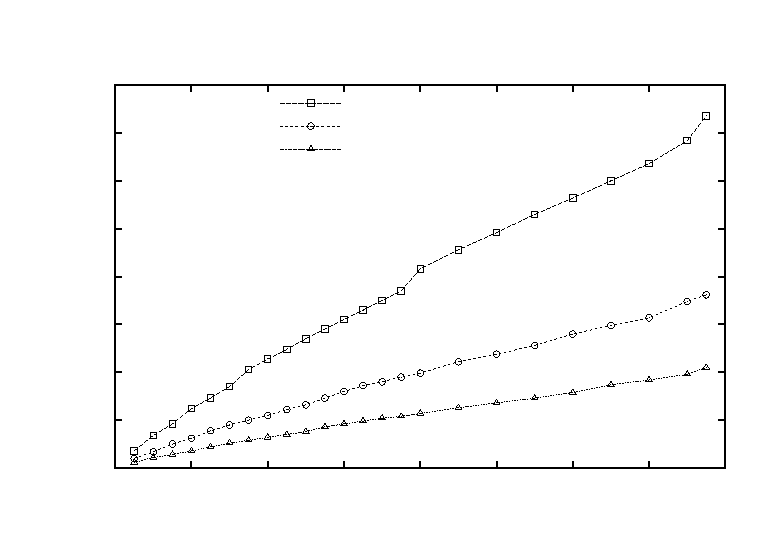
\includegraphics{benchmark-cs-en-vm-peaks}}%
    \gplfronttext
  \end{picture}%
\endgroup

  \caption{
    A plot of virtual memory peaks of various \eppex{} configurations invoked on the subsets of Cs-En training data.
  }
  \label{fig:cs-en-vm-peaks}
\end{figure}

This observation inspired us to take a look onto the possibility of predicting the memory
demands of the epochal extraction.
Specifically, we were curious, if a virtual memory peak quickly determined by running
\eppex{} on some subset of the training data make it possible to predict the amount of
memory required to process the whole data.

For each batch of size $K$ with the virtual memory peak $vm_{K}$ we evaluated the predicted virtual
memory peak as: $pred_{K} = vm_{K} / K \times N$, where $N$ is the size of the whole
data.\footnote{Assuming the linear correlation, the ratio $vm_{K} / K$ is an estimation of the linear coefficient.}
We then calculated the error of prediction $pred_{K}$ as the normalized difference between
the prediction and true virtual memory peak $vm_{real}$: $err_{K} = (pred_{K} - vm_{real}) / vm_{real}$.
\Fref{fig:cs-en-vm-peak-prediction} presents the error values for subsets of increasing size
expressed as percentages.

\begin{figure}[!htb]
  \centering
  % GNUPLOT: LaTeX picture with Postscript
\begingroup
  \makeatletter
  \providecommand\color[2][]{%
    \GenericError{(gnuplot) \space\space\space\@spaces}{%
      Package color not loaded in conjunction with
      terminal option `colourtext'%
    }{See the gnuplot documentation for explanation.%
    }{Either use 'blacktext' in gnuplot or load the package
      color.sty in LaTeX.}%
    \renewcommand\color[2][]{}%
  }%
  \providecommand\includegraphics[2][]{%
    \GenericError{(gnuplot) \space\space\space\@spaces}{%
      Package graphicx or graphics not loaded%
    }{See the gnuplot documentation for explanation.%
    }{The gnuplot epslatex terminal needs graphicx.sty or graphics.sty.}%
    \renewcommand\includegraphics[2][]{}%
  }%
  \providecommand\rotatebox[2]{#2}%
  \@ifundefined{ifGPcolor}{%
    \newif\ifGPcolor
    \GPcolorfalse
  }{}%
  \@ifundefined{ifGPblacktext}{%
    \newif\ifGPblacktext
    \GPblacktexttrue
  }{}%
  % define a \g@addto@macro without @ in the name:
  \let\gplgaddtomacro\g@addto@macro
  % define empty templates for all commands taking text:
  \gdef\gplbacktext{}%
  \gdef\gplfronttext{}%
  \makeatother
  \ifGPblacktext
    % no textcolor at all
    \def\colorrgb#1{}%
    \def\colorgray#1{}%
  \else
    % gray or color?
    \ifGPcolor
      \def\colorrgb#1{\color[rgb]{#1}}%
      \def\colorgray#1{\color[gray]{#1}}%
      \expandafter\def\csname LTw\endcsname{\color{white}}%
      \expandafter\def\csname LTb\endcsname{\color{black}}%
      \expandafter\def\csname LTa\endcsname{\color{black}}%
      \expandafter\def\csname LT0\endcsname{\color[rgb]{1,0,0}}%
      \expandafter\def\csname LT1\endcsname{\color[rgb]{0,1,0}}%
      \expandafter\def\csname LT2\endcsname{\color[rgb]{0,0,1}}%
      \expandafter\def\csname LT3\endcsname{\color[rgb]{1,0,1}}%
      \expandafter\def\csname LT4\endcsname{\color[rgb]{0,1,1}}%
      \expandafter\def\csname LT5\endcsname{\color[rgb]{1,1,0}}%
      \expandafter\def\csname LT6\endcsname{\color[rgb]{0,0,0}}%
      \expandafter\def\csname LT7\endcsname{\color[rgb]{1,0.3,0}}%
      \expandafter\def\csname LT8\endcsname{\color[rgb]{0.5,0.5,0.5}}%
    \else
      % gray
      \def\colorrgb#1{\color{black}}%
      \def\colorgray#1{\color[gray]{#1}}%
      \expandafter\def\csname LTw\endcsname{\color{white}}%
      \expandafter\def\csname LTb\endcsname{\color{black}}%
      \expandafter\def\csname LTa\endcsname{\color{black}}%
      \expandafter\def\csname LT0\endcsname{\color{black}}%
      \expandafter\def\csname LT1\endcsname{\color{black}}%
      \expandafter\def\csname LT2\endcsname{\color{black}}%
      \expandafter\def\csname LT3\endcsname{\color{black}}%
      \expandafter\def\csname LT4\endcsname{\color{black}}%
      \expandafter\def\csname LT5\endcsname{\color{black}}%
      \expandafter\def\csname LT6\endcsname{\color{black}}%
      \expandafter\def\csname LT7\endcsname{\color{black}}%
      \expandafter\def\csname LT8\endcsname{\color{black}}%
    \fi
  \fi
  \setlength{\unitlength}{0.0500bp}%
  \begin{picture}(7200.00,5040.00)%
    \gplgaddtomacro\gplbacktext{%
      \csname LTb\endcsname%
      \put(814,704){\makebox(0,0)[r]{\strut{}-10}}%
      \put(814,1112){\makebox(0,0)[r]{\strut{} 0}}%
      \put(814,1521){\makebox(0,0)[r]{\strut{} 10}}%
      \put(814,1929){\makebox(0,0)[r]{\strut{} 20}}%
      \put(814,2337){\makebox(0,0)[r]{\strut{} 30}}%
      \put(814,2746){\makebox(0,0)[r]{\strut{} 40}}%
      \put(814,3154){\makebox(0,0)[r]{\strut{} 50}}%
      \put(814,3562){\makebox(0,0)[r]{\strut{} 60}}%
      \put(814,3971){\makebox(0,0)[r]{\strut{} 70}}%
      \put(814,4379){\makebox(0,0)[r]{\strut{} 80}}%
      \put(946,484){\makebox(0,0){\strut{} 0}}%
      \put(1532,484){\makebox(0,0){\strut{} 10}}%
      \put(2117,484){\makebox(0,0){\strut{} 20}}%
      \put(2703,484){\makebox(0,0){\strut{} 30}}%
      \put(3289,484){\makebox(0,0){\strut{} 40}}%
      \put(3875,484){\makebox(0,0){\strut{} 50}}%
      \put(4460,484){\makebox(0,0){\strut{} 60}}%
      \put(5046,484){\makebox(0,0){\strut{} 70}}%
      \put(5632,484){\makebox(0,0){\strut{} 80}}%
      \put(6217,484){\makebox(0,0){\strut{} 90}}%
      \put(6803,484){\makebox(0,0){\strut{} 100}}%
      \put(176,2541){\rotatebox{-270}{\makebox(0,0){\strut{}error of VM peak prediction (\%)}}}%
      \put(3874,154){\makebox(0,0){\strut{}training data subset size (\%)}}%
      \put(3874,4709){\makebox(0,0){\strut{}Cs-En: training data subset size vs. error of VM peak prediction}}%
    }%
    \gplgaddtomacro\gplfronttext{%
      \csname LTb\endcsname%
      \put(2398,4206){\makebox(0,0)[r]{\strut{}eppex zero}}%
      \csname LTb\endcsname%
      \put(2398,3986){\makebox(0,0)[r]{\strut{}eppex def.}}%
      \csname LTb\endcsname%
      \put(2398,3766){\makebox(0,0)[r]{\strut{}eppex 0:n}}%
    }%
    \gplbacktext
    \put(0,0){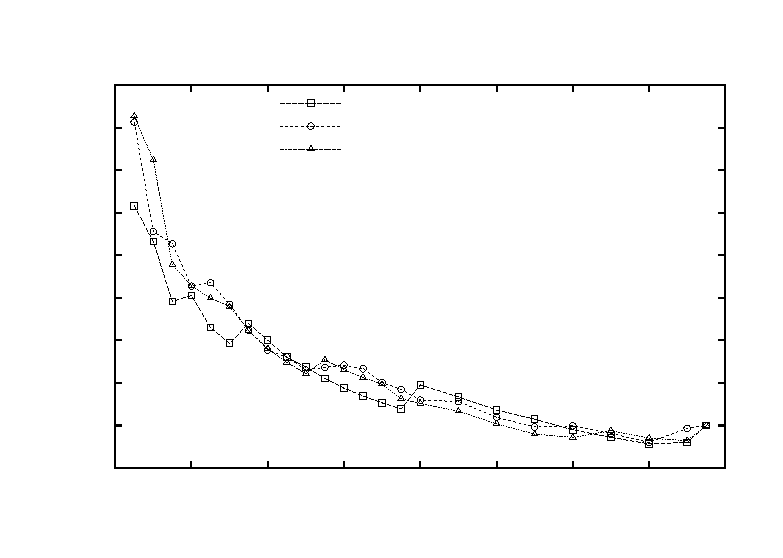
\includegraphics{predict-cs-en-vm-peaks}}%
    \gplfronttext
  \end{picture}%
\endgroup

  \caption{
    Error of virtual memory peak predictions based on the partial runs of various \eppex{} configurations
    invoked on the subsets of Cs-En training data.
  }
  \label{fig:cs-en-vm-peak-prediction}
\end{figure}

With all three configurations, the prediction errors had a very similar course: predictions on small
subsets were strongly overestimated, but the error continually declined with the increasing ratio
of the training data used.
A decent prediction, overestimating the total VM peak by no more than 20\%, was possible based on $1/4$
of the training data.

\subsection{Fr-En dataset}

The French-English training data contained only a single factor: input token in lowercase.
There were on average 30~French and 25.5~English tokens per sentence in the whole data,
but in most of the batches the averages were below these values (down to 25.5~tokens
per sentence in the case of French and 24~tokens per sentence in the case of English).
Compared to the Cs-En dataset, the sentences were on average almost twice as long and
likewise the phrase-pairs-per-sentence ratio was twice as large, almost~46 in the case of
unpruned phrase table.

In the case of Fr-En data, we decided to point out the differences between the memory demands
and the output sizes of three \eppex{} configurations instantiated with a separate Lossy Counting
instances for each phrase length, as two of them have the same error margin and two of them
prune with the same negative limit.

\Fref{fig:fr-en-vm-peaks} illustrates the influence of error margin on \eppex{} memory demands
(the complete figures are part of \Tref{fr-en-memory-benchmarking}).
Both \emph{eppex 0:n} and \emph{eppex 1:n+1} configurations have the same error margins and
their memory demands closely follow each other, with the latter having a bit lower memory
peaks, because of the harsher pruning.

\begin{figure}[!htb]
  \centering
  % GNUPLOT: LaTeX picture with Postscript
\begingroup
  \makeatletter
  \providecommand\color[2][]{%
    \GenericError{(gnuplot) \space\space\space\@spaces}{%
      Package color not loaded in conjunction with
      terminal option `colourtext'%
    }{See the gnuplot documentation for explanation.%
    }{Either use 'blacktext' in gnuplot or load the package
      color.sty in LaTeX.}%
    \renewcommand\color[2][]{}%
  }%
  \providecommand\includegraphics[2][]{%
    \GenericError{(gnuplot) \space\space\space\@spaces}{%
      Package graphicx or graphics not loaded%
    }{See the gnuplot documentation for explanation.%
    }{The gnuplot epslatex terminal needs graphicx.sty or graphics.sty.}%
    \renewcommand\includegraphics[2][]{}%
  }%
  \providecommand\rotatebox[2]{#2}%
  \@ifundefined{ifGPcolor}{%
    \newif\ifGPcolor
    \GPcolorfalse
  }{}%
  \@ifundefined{ifGPblacktext}{%
    \newif\ifGPblacktext
    \GPblacktexttrue
  }{}%
  % define a \g@addto@macro without @ in the name:
  \let\gplgaddtomacro\g@addto@macro
  % define empty templates for all commands taking text:
  \gdef\gplbacktext{}%
  \gdef\gplfronttext{}%
  \makeatother
  \ifGPblacktext
    % no textcolor at all
    \def\colorrgb#1{}%
    \def\colorgray#1{}%
  \else
    % gray or color?
    \ifGPcolor
      \def\colorrgb#1{\color[rgb]{#1}}%
      \def\colorgray#1{\color[gray]{#1}}%
      \expandafter\def\csname LTw\endcsname{\color{white}}%
      \expandafter\def\csname LTb\endcsname{\color{black}}%
      \expandafter\def\csname LTa\endcsname{\color{black}}%
      \expandafter\def\csname LT0\endcsname{\color[rgb]{1,0,0}}%
      \expandafter\def\csname LT1\endcsname{\color[rgb]{0,1,0}}%
      \expandafter\def\csname LT2\endcsname{\color[rgb]{0,0,1}}%
      \expandafter\def\csname LT3\endcsname{\color[rgb]{1,0,1}}%
      \expandafter\def\csname LT4\endcsname{\color[rgb]{0,1,1}}%
      \expandafter\def\csname LT5\endcsname{\color[rgb]{1,1,0}}%
      \expandafter\def\csname LT6\endcsname{\color[rgb]{0,0,0}}%
      \expandafter\def\csname LT7\endcsname{\color[rgb]{1,0.3,0}}%
      \expandafter\def\csname LT8\endcsname{\color[rgb]{0.5,0.5,0.5}}%
    \else
      % gray
      \def\colorrgb#1{\color{black}}%
      \def\colorgray#1{\color[gray]{#1}}%
      \expandafter\def\csname LTw\endcsname{\color{white}}%
      \expandafter\def\csname LTb\endcsname{\color{black}}%
      \expandafter\def\csname LTa\endcsname{\color{black}}%
      \expandafter\def\csname LT0\endcsname{\color{black}}%
      \expandafter\def\csname LT1\endcsname{\color{black}}%
      \expandafter\def\csname LT2\endcsname{\color{black}}%
      \expandafter\def\csname LT3\endcsname{\color{black}}%
      \expandafter\def\csname LT4\endcsname{\color{black}}%
      \expandafter\def\csname LT5\endcsname{\color{black}}%
      \expandafter\def\csname LT6\endcsname{\color{black}}%
      \expandafter\def\csname LT7\endcsname{\color{black}}%
      \expandafter\def\csname LT8\endcsname{\color{black}}%
    \fi
  \fi
  \setlength{\unitlength}{0.0500bp}%
  \begin{picture}(7200.00,5040.00)%
    \gplgaddtomacro\gplbacktext{%
      \csname LTb\endcsname%
      \put(814,704){\makebox(0,0)[r]{\strut{} 0}}%
      \put(814,1072){\makebox(0,0)[r]{\strut{} 5}}%
      \put(814,1439){\makebox(0,0)[r]{\strut{} 10}}%
      \put(814,1807){\makebox(0,0)[r]{\strut{} 15}}%
      \put(814,2174){\makebox(0,0)[r]{\strut{} 20}}%
      \put(814,2542){\makebox(0,0)[r]{\strut{} 25}}%
      \put(814,2909){\makebox(0,0)[r]{\strut{} 30}}%
      \put(814,3277){\makebox(0,0)[r]{\strut{} 35}}%
      \put(814,3644){\makebox(0,0)[r]{\strut{} 40}}%
      \put(814,4012){\makebox(0,0)[r]{\strut{} 45}}%
      \put(814,4379){\makebox(0,0)[r]{\strut{} 50}}%
      \put(946,484){\makebox(0,0){\strut{} 0}}%
      \put(1678,484){\makebox(0,0){\strut{} 5}}%
      \put(2410,484){\makebox(0,0){\strut{} 10}}%
      \put(3142,484){\makebox(0,0){\strut{} 15}}%
      \put(3875,484){\makebox(0,0){\strut{} 20}}%
      \put(4607,484){\makebox(0,0){\strut{} 25}}%
      \put(5339,484){\makebox(0,0){\strut{} 30}}%
      \put(6071,484){\makebox(0,0){\strut{} 35}}%
      \put(6803,484){\makebox(0,0){\strut{} 40}}%
      \put(176,2541){\rotatebox{-270}{\makebox(0,0){\strut{}virtual memory peak (GB)}}}%
      \put(3874,154){\makebox(0,0){\strut{}input size in sentences (M)}}%
      \put(3874,4709){\makebox(0,0){\strut{}Fr-En: corpus size vs. VM peak}}%
    }%
    \gplgaddtomacro\gplfronttext{%
      \csname LTb\endcsname%
      \put(2530,4206){\makebox(0,0)[r]{\strut{}eppex 0:n}}%
      \csname LTb\endcsname%
      \put(2530,3986){\makebox(0,0)[r]{\strut{}eppex 1:n+1}}%
      \csname LTb\endcsname%
      \put(2530,3766){\makebox(0,0)[r]{\strut{}eppex 1:n+2}}%
    }%
    \gplbacktext
    \put(0,0){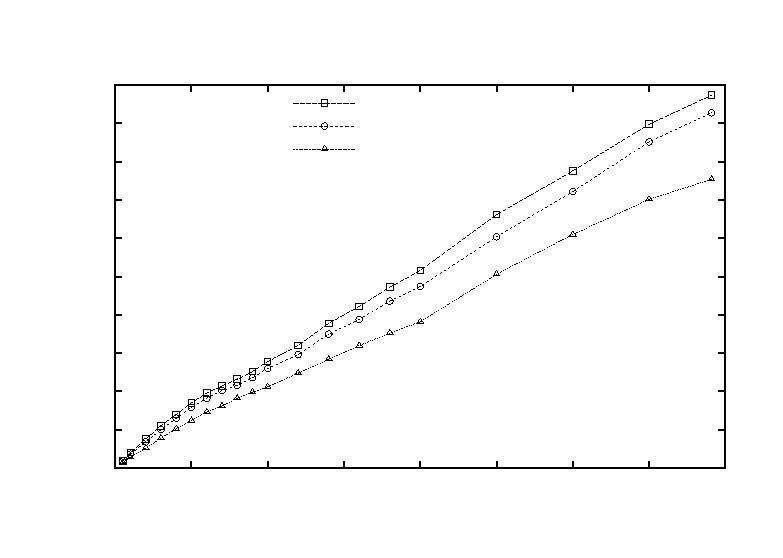
\includegraphics{benchmark-fr-en-vm-peaks}}%
    \gplfronttext
  \end{picture}%
\endgroup

  \caption{
    A plot of virtual memory peaks of three \eppex{} configurations invoked on subsets of Fr-En training data.
  }
  \label{fig:fr-en-vm-peaks}
\end{figure}

Despite that \emph{eppex 0:n} and \emph{eppex 1:n+1} have a similar memory demands, their outputs
differ significantly, as \Fref{fig:fr-en-phrase-table-sizes} presents (the complete figures are part
of \Tref{fr-en-output-size-benchmarking}).
The \emph{eppex 1:n+1} configuration pruned off all the singletons, so it consistently
produced phrase tables substantially smaller than the \emph{eppex 0:n} configuration.
In fact, the degree of pruning of \emph{eppex 1:n+1} is very close to the \emph{eppex 1:n+2} configuration,
because in both cases it is determined by the common negative limit.

\begin{figure}[!htb]
  \centering
  % GNUPLOT: LaTeX picture with Postscript
\begingroup
  \makeatletter
  \providecommand\color[2][]{%
    \GenericError{(gnuplot) \space\space\space\@spaces}{%
      Package color not loaded in conjunction with
      terminal option `colourtext'%
    }{See the gnuplot documentation for explanation.%
    }{Either use 'blacktext' in gnuplot or load the package
      color.sty in LaTeX.}%
    \renewcommand\color[2][]{}%
  }%
  \providecommand\includegraphics[2][]{%
    \GenericError{(gnuplot) \space\space\space\@spaces}{%
      Package graphicx or graphics not loaded%
    }{See the gnuplot documentation for explanation.%
    }{The gnuplot epslatex terminal needs graphicx.sty or graphics.sty.}%
    \renewcommand\includegraphics[2][]{}%
  }%
  \providecommand\rotatebox[2]{#2}%
  \@ifundefined{ifGPcolor}{%
    \newif\ifGPcolor
    \GPcolorfalse
  }{}%
  \@ifundefined{ifGPblacktext}{%
    \newif\ifGPblacktext
    \GPblacktexttrue
  }{}%
  % define a \g@addto@macro without @ in the name:
  \let\gplgaddtomacro\g@addto@macro
  % define empty templates for all commands taking text:
  \gdef\gplbacktext{}%
  \gdef\gplfronttext{}%
  \makeatother
  \ifGPblacktext
    % no textcolor at all
    \def\colorrgb#1{}%
    \def\colorgray#1{}%
  \else
    % gray or color?
    \ifGPcolor
      \def\colorrgb#1{\color[rgb]{#1}}%
      \def\colorgray#1{\color[gray]{#1}}%
      \expandafter\def\csname LTw\endcsname{\color{white}}%
      \expandafter\def\csname LTb\endcsname{\color{black}}%
      \expandafter\def\csname LTa\endcsname{\color{black}}%
      \expandafter\def\csname LT0\endcsname{\color[rgb]{1,0,0}}%
      \expandafter\def\csname LT1\endcsname{\color[rgb]{0,1,0}}%
      \expandafter\def\csname LT2\endcsname{\color[rgb]{0,0,1}}%
      \expandafter\def\csname LT3\endcsname{\color[rgb]{1,0,1}}%
      \expandafter\def\csname LT4\endcsname{\color[rgb]{0,1,1}}%
      \expandafter\def\csname LT5\endcsname{\color[rgb]{1,1,0}}%
      \expandafter\def\csname LT6\endcsname{\color[rgb]{0,0,0}}%
      \expandafter\def\csname LT7\endcsname{\color[rgb]{1,0.3,0}}%
      \expandafter\def\csname LT8\endcsname{\color[rgb]{0.5,0.5,0.5}}%
    \else
      % gray
      \def\colorrgb#1{\color{black}}%
      \def\colorgray#1{\color[gray]{#1}}%
      \expandafter\def\csname LTw\endcsname{\color{white}}%
      \expandafter\def\csname LTb\endcsname{\color{black}}%
      \expandafter\def\csname LTa\endcsname{\color{black}}%
      \expandafter\def\csname LT0\endcsname{\color{black}}%
      \expandafter\def\csname LT1\endcsname{\color{black}}%
      \expandafter\def\csname LT2\endcsname{\color{black}}%
      \expandafter\def\csname LT3\endcsname{\color{black}}%
      \expandafter\def\csname LT4\endcsname{\color{black}}%
      \expandafter\def\csname LT5\endcsname{\color{black}}%
      \expandafter\def\csname LT6\endcsname{\color{black}}%
      \expandafter\def\csname LT7\endcsname{\color{black}}%
      \expandafter\def\csname LT8\endcsname{\color{black}}%
    \fi
  \fi
  \setlength{\unitlength}{0.0500bp}%
  \begin{picture}(7200.00,5040.00)%
    \gplgaddtomacro\gplbacktext{%
      \csname LTb\endcsname%
      \put(946,704){\makebox(0,0)[r]{\strut{} 0}}%
      \put(946,1317){\makebox(0,0)[r]{\strut{} 50}}%
      \put(946,1929){\makebox(0,0)[r]{\strut{} 100}}%
      \put(946,2542){\makebox(0,0)[r]{\strut{} 150}}%
      \put(946,3154){\makebox(0,0)[r]{\strut{} 200}}%
      \put(946,3767){\makebox(0,0)[r]{\strut{} 250}}%
      \put(946,4379){\makebox(0,0)[r]{\strut{} 300}}%
      \put(1078,484){\makebox(0,0){\strut{} 0}}%
      \put(1794,484){\makebox(0,0){\strut{} 5}}%
      \put(2509,484){\makebox(0,0){\strut{} 10}}%
      \put(3225,484){\makebox(0,0){\strut{} 15}}%
      \put(3941,484){\makebox(0,0){\strut{} 20}}%
      \put(4656,484){\makebox(0,0){\strut{} 25}}%
      \put(5372,484){\makebox(0,0){\strut{} 30}}%
      \put(6087,484){\makebox(0,0){\strut{} 35}}%
      \put(6803,484){\makebox(0,0){\strut{} 40}}%
      \put(176,2541){\rotatebox{-270}{\makebox(0,0){\strut{}phrase table size in phrase pairs (M)}}}%
      \put(3940,154){\makebox(0,0){\strut{}input size in sentences (M)}}%
      \put(3940,4709){\makebox(0,0){\strut{}Fr-En: corpus size vs. phrase table size}}%
    }%
    \gplgaddtomacro\gplfronttext{%
      \csname LTb\endcsname%
      \put(2662,4206){\makebox(0,0)[r]{\strut{}eppex 0:n}}%
      \csname LTb\endcsname%
      \put(2662,3986){\makebox(0,0)[r]{\strut{}eppex 1:n+1}}%
      \csname LTb\endcsname%
      \put(2662,3766){\makebox(0,0)[r]{\strut{}eppex 1:n+2}}%
    }%
    \gplbacktext
    \put(0,0){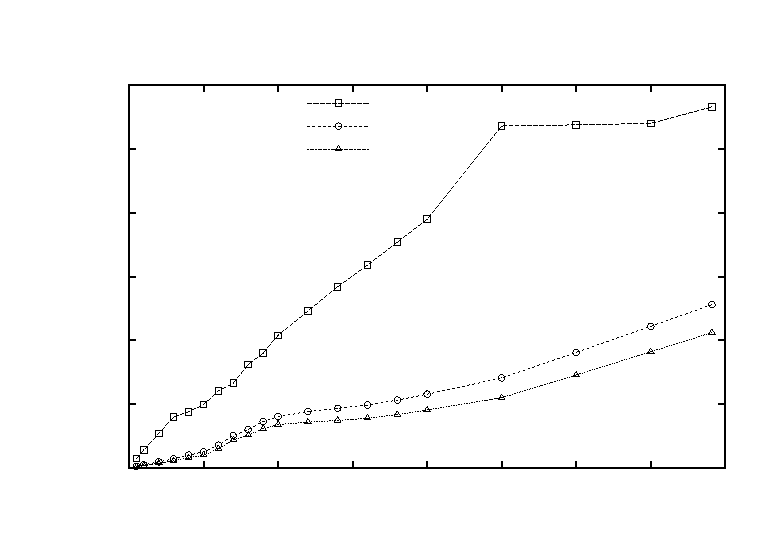
\includegraphics{benchmark-fr-en-phrase-table-sizes}}%
    \gplfronttext
  \end{picture}%
\endgroup

  \caption{
    A plot of phrase table sizes obtained with three \eppex{} configurations invoked on subsets of Fr-En training data.
  }
  \label{fig:fr-en-phrase-table-sizes}
\end{figure}

One more observable phenomenon is the clearly visible plateau in the plot of phrase table sizes
obtained by the \emph{eppex 0:n} configuration on the range of input sizes from 25~M to 35~M parallel sentences.
A quick examination of the figures in \Tref{fr-en-output-size-benchmarking} confirms that, indeed, with
the \emph{eppex 0:n} configuration, 268~M of phrase pairs is extracted from 25~M of parallel sentences,
but only 1~M more is extracted from the additional 5~M of sentences and 2~M more from the additional
10~M of sentences.

The origin of this peculiarity lies in the great amount of phrase pairs with counts in the error
margin zone, i.e. phrase pairs that are neither guaranteed to be removed nor retained.
If such a phrase pair happened to be extracted from a batch of a certain size, but has no more
additional occurrences in the batch of increased size, then the likelihood of its extraction
goes down.

Since our corpus was created from a several smaller corpora and we did not shuffle the sentences,
it is likely that the distribution of extracted phrase pairs rapidly changed as a result of data
coming from a different parallel corpus and, consequently, the amount of phrase pairs in the error zone,
that happened to be pruned, massively increased.

Nevertheless, the definition of Lossy Counting limits guarantees that,
whenever the limits are fixed, adding more items to the input stream results in at least
as many phrase pairs extracted as from the non extended stream.
